%\documentclass[oneside,numbers,spanish,a4paper]{ezthesis}
\documentclass[twoside,spanish,a4paper]{ezthesis}
%\documentclass[oneside,authoryear,draft,spanish]{ezthesis}
%\documentclass[oneside,authoryear,draftmarks,spanish]{ezthesis}
%% # Opciones disponibles para el documento #
%%
%% Las opciones con un (*) son las opciones predeterminadas.
%%
%% Modo de compilar:
%%   draft            - borrador con marcas de fecha y sin im'agenes
%%   draftmarks       - borrador con marcas de fecha y con im'agenes
%%   final (*)        - version final de la tesis
%%
%% Tama'no de papel:
%%   letterpaper (*)  - tama'no carta (Am'erica)
%%   a4paper          - tama'no A4    (Europa)
%%
%% Formato de impresi'on:
%%   oneside          - hojas impresas por un solo lado
%%   twoside (*)      - hijas impresas por ambos lados
%%
%% Tama'no de letra:
%%   10pt, 11pt, o 12pt (*)
%%
%% Espaciado entre renglones:
%%   singlespace      - espacio sencillo
%%   onehalfspace (*) - espacio de 1.5
%%   doublespace      - a doble espacio
%%
%% Formato de las referencias bibliogr'aficas:
%%   numbers          - numeradas, p.e. [1]
%%   authoryear (*)   - por autor y a'no, p.e. (Newton, 1997)
%%
%% Opciones adicionales:
%%   spanish         - tesis escrita en espa'nol
%%
%% Desactivar opciones especiales:
%%   nobibtoc   - no incluir la bibiolgraf'ia en el 'Indice general
%%   nofancyhdr - no incluir "fancyhdr" para producir los encabezados
%%   nocolors   - no incluir "xcolor" para producir ligas con colores
%%   nographicx - no incluir "graphicx" para insertar gr'aficos
%%   nonatbib   - no incluir "natbib" para administrar la bibliograf'ia

%% Paquetes adicionales requeridos se pueden agregar tambi'en aqu'i.
%% Por ejemplo:
\usepackage{graphics}
\usepackage{graphicx}
\usepackage{float}
\usepackage{rotating}
\usepackage[export]{adjustbox}
\usepackage{tablefootnote}

\usepackage{subfig}
\usepackage{multirow}
\usepackage[activeacute,spanish]{babel}
\usepackage[utf8]{inputenc}
\usepackage{amsmath}
\usepackage{mathtools}
\usepackage{amsmath,amssymb,amsfonts,latexsym,cancel}
\usepackage{rawfonts}
\usepackage{pictexwd}
\usepackage{float}
\usepackage{mdwlist}
\usepackage{booktabs}
\usepackage{graphicx}
\numberwithin{equation}{section}
%paquete para diagramas
\usepackage[all]{xy}
\usepackage{mathrsfs}
%\usepackage{tikz}
%\usetikzlibrary{3d}
%\usepackage{tikz-3dplot}
\usepackage[thinlines]{easytable}
\usepackage[none]{hyphenat}
%Configuracion codigo c++
\usepackage{listings}
\usepackage[T1]{fontenc}
\usepackage{times}
\usepackage{color}

\usepackage{eulervm}
\newcommand{\be}{\begin{equation}}
\newcommand{\ee}{\end{equation}}
\newcommand{\bce}{\begin{center}}
\newcommand{\ece}{\end{center}}

\definecolor{lightblue}{rgb}{0, 0.7, .7}
\definecolor{gray97}{gray}{.97}
\definecolor{gray75}{gray}{.75}
\definecolor{gray45}{gray}{.45}
\lstset{ frame=Ltb,
framerule=0pt,
aboveskip=0.5cm,
framextopmargin=3pt,
framexbottommargin=3pt,
framexleftmargin=0.4cm,
framesep=0pt,
rulesep=.4pt,
backgroundcolor=\color{gray97},
rulesepcolor=\color{black},
%
stringstyle=\ttfamily,
showstringspaces = false,
basicstyle=\tiny\ttfamily,
commentstyle=\color{gray45},
keywordstyle=\bfseries,
%
numbers=left,
numbersep=15pt,
numberstyle=\tiny,
numberfirstline = false,
breaklines=true,
}
% minimizar fragmentado de listados
\lstnewenvironment{listing}[1][]
{\lstset{#1}\pagebreak[0]}{\pagebreak[0]}

\lstdefinestyle{consola}
{basicstyle=\scriptsize\bf\ttfamily,
%backgroundcolor=\color{gray75},
}

\lstdefinestyle{C}
{language=C,
}

\lstdefinestyle{customc}{
  belowcaptionskip=1\baselineskip,
  breaklines=true,
  frame=L,
  xleftmargin=\parindent,
  language=C,
  showstringspaces=false,
  basicstyle=\footnotesize\ttfamily,
  keywordstyle=\bfseries\color{green!40!black},
  commentstyle=\itshape\color{purple!40!black},
  identifierstyle=\color{blue},
  stringstyle=\color{orange},
}

\lstdefinestyle{customasm}{
  belowcaptionskip=1\baselineskip,
  frame=L,
  xleftmargin=\parindent,
  language=[x86masm]Assembler,
  basicstyle=\footnotesize\ttfamily,
  commentstyle=\itshape\color{purple!40!black},
}

\lstset{style=customc,basicstyle=\small}
%

%\usepackage{ccaption}%Cambia el formato de los pie de foto o tabla
%\captionnamefont{\bfseries}
%\captiontitlefont{\small}
%\captiondelim{:\ }
%\hangcaption
%\addto\captionsspanish{
%	\def\tablename{Tabla}
%}
\usepackage[labelfont=bf]{caption}
\makeatletter
\def\tagform@#1{\maketag@@@{(\ignorespaces\textbf{#1}\unskip\@@italiccorr)}}
\renewcommand{\eqref}[1]{\textup{{\normalfont(\ref{#1}}\normalfont)}}
\makeatother
\usepackage{natbib}
\setcitestyle{aysep={},yysep={;}}
%\bibliographystyle{spbasic}
%%##################################################################################################################################
%% # Datos del documento #
%% Nota que los acentos se deben escribir: \'a, \'e, \'i, etc.
%% La letra n con tilde es: \~n.

\author{Ignacio Alberto Apablaza Benavides}
\title{}
\degree{Magíster en Ciencias de la Ingeniería Mecánica }
\supervisor{Ph.D. Franco Perazzo Maggi}
\correferent{Ph.D. Oscar Orellana Estay}
\correferentextern{Ph.D. - }
\institution{UNIVERSIDAD TÉCNICA FEDERICO SANTA MARÍA}
\faculty{Escuela de Ingeniería y Ciencias}
\department{DEPARTAMENTO DE INGENIERÍA MECÁNICA}
\city{VALPARAÍSO }
\country{CHILE }

%% # Márgenes del documento #
%% 
%% Quitar el comentario en la siguiente linea para austar los m'argenes del
%% documento. Leer la documentaci'on de "geometry" para m'as informaci'on.

%\geometry{top=30mm,bottom=30mm,inner=40mm,outer=30mm}

%% El siguiente comando agrega ligas activas en el documento para las
%% referencias cruzadas y citas bibliogr'aficas. Tiene que ser *la 'ultima*
%% instrucci'on antes de \begin{document}.
\usepackage{titlesec}
\usepackage{etoolbox}

\makeatletter
\patchcmd{\ttlh@hang}{\parindent\z@}{\parindent\z@\leavevmode}{}{}
\patchcmd{\ttlh@hang}{\noindent}{}{}{}
\makeatother

\titleformat{\chapter}[display]
{\normalfont\huge\bfseries}{\chaptertitlename\ \thechapter}{20pt}{\Huge}
\titlespacing*{\chapter}{0pt}{0pt}{20pt}
\hyperlinking
\begin{document}
\renewcommand{\listtablename}{Índice de tablas}
\renewcommand{\tablename}{Tabla} 
\pagenumbering{roman}
\sloppy 

%% En esta secci'on se describe la estructura del documento de la tesis.
%% Consulta los reglamentos de tu universidad para determinar el orden
%% y la cantidad de secciones que debes de incluir.

%% # Portada de la tesis #
%\include{Portada/anteportada}
%\include{blanco}
%% ## Construye tu propia portada ##
%% 
%% Una portada se conforma por una secuencia de "Blocks" que incluyen
%% piezas individuales de informaci'on. Un "Block" puede incluir, por
%% ejemplo, el t'itulo del documento, una im'agen (logotipo de la universidad),
%% el nombre del autor, nombre del supervisor, u cualquier otra pieza de
%% informaci'on.
%%
%% Cada "Block" aparece centrado horizontalmente en la p'agina y,
%% verticalmente, todos los "Blocks" se distruyen de manera uniforme 
%% a lo largo de p'agina.
%%
%% Nota tambi'en que, dentro de un mismo "Block" se pueden cortar
%% lineas usando el comando \\
%%
%% El tama'no del texto dentro de un "Block" se puede modificar usando uno de
%% los comandos:
%%   \small      \LARGE
%%   \large      \huge
%%   \Large      \Huge
%%
%% Y el tipo de letra se puede modificar usando:
%%   \bfseries - negritas
%%   \itshape  - it'alicas
%%   \scshape  - small caps
%%   \slshape  - slanted
%%   \sffamily - sans serif
%%
%% Para producir plantillas generales, la informaci'on que ha sido inclu'ida
%% en el archivo principal "tesis.tex" se puede accesar aqu'i usando:
%%   \insertauthor
%%   \inserttitle
%%   \insertsupervisor
%%	 \insertcorreferent
%%   \insertinstitution
%%   \insertdegree
%%   \insertfaculty
%%   \insertdepartment
%%	 \insertcity
%%	 \insertcountry
%%   \insertsubmitdate

\begin{titlepage}
	\TitleBlock[\vspace{-1.5in}]{
		\bfseries\insertinstitution}
	\TitleBlock[\vspace{-0.05in}]{
		\insertdepartment}
	\TitleBlock[\vspace{-0.05in}]{
		\insertcity - \insertcountry}
	
	%\TitleBlock[\vspace{-1.5 in}]{\includegraphics[height=4cm]{Imagenes/utfsm_logo}}
	\TitleBlock[\vspace{0.5 in}]{\includegraphics[height=4cm]{Imagenes/utfsm_logo}}
	\TitleBlock[\vspace{0.5in}]{
		\small\scshape\bfseries\inserttitle}
	\TitleBlock[\vspace{0.5in}]{
		\small\scshape\bfseries\insertauthor}
    \TitleBlock[\vspace{0.5in}]{
    	TESIS DE GRADO PARA OPTAR AL GRADO DE: \\
    	\textbf{MAGÍSTER EN CIENCIAS DE LA INGENIERÍA MECÁNICA}\\
	    Y AL TITULO DE:\\
	    \textbf{INGENIERO CIVIL MECÁNICO}}
		\begin{minipage}{0.99\textwidth}
			\TitleBlock[\vspace{0.5in}]{
				\begin{center}
					Profesor Guia: \insertsupervisor
				\end{center}}\vspace{-9mm}
			\TitleBlock{
				\begin{center}
					Profesor Correferente: \insertcorreferent
				\end{center}}\vspace{-9mm}
			\TitleBlock{
				\begin{center}
					Evaluador Externo: \insertcorreferentextern
			\end{center}}
		\end{minipage}
		\TitleBlock{MARZO - \insertsubmitdate}
\end{titlepage}

%% Nota 1
%% Se puede agregar un escudo o logotipo en un "Block" como:
%%   \TitleBlock{\includegraphics[height=4cm]{escudo_uni}}
%% y teniendo un archivo "escudo_uni.pdf", "escudo_uni.png" o "escudo_uni.jpg"
%% en alg'un lugar donde LaTeX lo pueda encontrar.

%% Nota 2:
%% Normalmente, el espacio entre "Blocks" se extiende de modo que el
%% contenido se reparte uniformemente sobre toda la p'agina. Este
%% comportamiento se puede modificar para mantener fijo, por ejemplo, el
%% espacio entre un par de "Blocks". Escribiendo:
%%   \TitleBlock{Bloque 1}
%%   \TitleBlock[\bigskip]{Bloque2}
%% se deja un espacio "grande" y de tama~no fijo entre el bloque 1 y 2.
%% Adem'as de \bigskip est'an tambi'en \smallskip y \medskip. Si necesitas
%% aun m'as control puedes usar tambi'en, por ejemplo, \vspace*{2cm}.



\include{blanco}
%% ## Construye tu propia portada ##
%% 
%% Una portada se conforma por una secuencia de "Blocks" que incluyen
%% piezas individuales de informaci'on. Un "Block" puede incluir, por
%% ejemplo, el t'itulo del documento, una im'agen (logotipo de la universidad),
%% el nombre del autor, nombre del supervisor, u cualquier otra pieza de
%% informaci'on.
%%
%% Cada "Block" aparece centrado horizontalmente en la p'agina y,
%% verticalmente, todos los "Blocks" se distruyen de manera uniforme 
%% a lo largo de p'agina.
%%
%% Nota tambi'en que, dentro de un mismo "Block" se pueden cortar
%% lineas usando el comando \\
%%
%% El tama'no del texto dentro de un "Block" se puede modificar usando uno de
%% los comandos:
%%   \small      \LARGE
%%   \large      \huge
%%   \Large      \Huge
%%
%% Y el tipo de letra se puede modificar usando:
%%   \bfseries - negritas
%%   \itshape  - it'alicas
%%   \scshape  - small caps
%%   \slshape  - slanted
%%   \sffamily - sans serif
%%
%% Para producir plantillas generales, la informaci'on que ha sido inclu'ida
%% en el archivo principal "tesis.tex" se puede accesar aqu'i usando:
%%   \insertauthor
%%   \inserttitle
%%   \insertsupervisor
%%	 \insertcorreferent
%%   \insertinstitution
%%   \insertdegree
%%   \insertfaculty
%%   \insertdepartment
%%	 \insertcity
%%	 \insertcountry
%%   \insertsubmitdate

\begin{titlepage}
	\TitleBlock[\vspace{-1.50in}]{
		\begin{flushleft}
			\small \scshape TÍTULO DE LA TESIS:
		\end{flushleft}
		}
	\TitleBlock[\vspace{0.00in}]{
		\small \textbf{Desarrollo de una metodología sin malla de Formulación fuerte utilizando funciones de forma tipo MAXENT }
		}
	\TitleBlock[\vspace{0.00in}]{
		\begin{flushleft}
			\small AUTOR:
		\end{flushleft}
		}
	\TitleBlock[\vspace{0.0in}]{
		\textbf{\insertauthor}
		}
    \TitleBlock[\vspace{1.0in}]{
    	\small TRABAJO DE TESIS, presentado en cumplimiento parcial de los requisitos para el Grado de \insertdegree de la Universidad T\'ecnica Federico Santa Mar\'ia.
		}
	\begin{minipage}{0.45\textwidth}
		\TitleBlock[\vspace{1in}]{
			\begin{center}
				\small \insertsupervisor
			\end{center}
			}
		\TitleBlock[\vspace{0.3in}]{
			\begin{center}
				\small \insertcorreferent
			\end{center}
			}
		\TitleBlock[\vspace{0.3in}]{
			\begin{center}
				\small \insertcorreferentextern
			\end{center}
		}
	\end{minipage}
	\begin{minipage}{0.45\textwidth}
%		\begin{figure}[H]
%			\centering
%			\vspace{0.7in}
%			\includegraphics[width=0.5\linewidth]{../firma_gers.png}
%		\end{figure}
%		\begin{figure}[H]
%			\centering
%			\vspace{-0.5in}
%			\includegraphics[width=0.5\linewidth]{../firma_olivier.png}
%		\end{figure}
%		\begin{figure}[H]
%			\centering
%			\vspace{-0.3in}
%			\includegraphics[width=0.7\linewidth]{../firma_elicer.png}
%		\end{figure}
		
				\TitleBlock[\vspace{1in}]{
					\begin{center}
						\small .............................
					\end{center}
					}
				\TitleBlock[\vspace{0.3in}]{
					\begin{center}
						\small .............................
					\end{center}
					}
				\TitleBlock[\vspace{0.3in}]{
					\begin{center}
						\small .............................
					\end{center}
					}
	\end{minipage}
	\TitleBlock[\vspace{1.5in}]{
		\\
		\small \insertcity\!, \insertcountry, MARZO - \insertsubmitdate		
		}
\end{titlepage}

%% Nota 1:
%% Se puede agregar un escudo o logotipo en un "Block" como:
%%   \TitleBlock{\includegraphics[height=4cm]{escudo_uni}}
%% y teniendo un archivo "escudo_uni.pdf", "escudo_uni.png" o "escudo_uni.jpg"
%% en alg'un lugar donde LaTeX lo pueda encontrar.

%% Nota 2:
%% Normalmente, el espacio entre "Blocks" se extiende de modo que el
%% contenido se reparte uniformemente sobre toda la p'agina. Este
%% comportamiento se puede modificar para mantener fijo, por ejemplo, el
%% espacio entre un par de "Blocks". Escribiendo:
%%   \TitleBlock{Bloque 1}
%%   \TitleBlock[\bigskip]{Bloque2}
%% se deja un espacio "grande" y de tama~no fijo entre el bloque 1 y 2.
%% Adem'as de \bigskip est'an tambi'en \smallskip y \medskip. Si necesitas
%% aun m'as control puedes usar tambi'en, por ejemplo, \vspace*{2cm}.

\include{blanco}

%% # Prefacios #
%% Por cada prefacio (p.e. agradecimientos, resumen, etc.) crear
%% un nuevo archivo e incluirlo aqu'i.
%% Para m'as detalles y un ejemplo mirar el archivo "gracias.tex".
%\newgeometry{top=30mm,bottom=30mm,inner=40mm,outer=30mm}
\thispagestyle{empty}
\vspace*{\fill}
\begin{quote}
	\raggedleft
	\emph{Cita}
	
	\bigskip
	\emph{Autor}
\end{quote}
\vspace*{\fill}



%% Las secciones del "prefacio" inician con el comando \prefacesection{T'itulo}
%% Este tipo de secciones *no* van numeradas, pero s'i aparecen en el 'indice.
%%
%% Si quieres agregar una secci'on que no vaya n'umerada y que *tampoco*
%% aparesca en el 'indice, usa entonces el comando \chapter*{T'itulo}
%%
%% Recuerda que aqu'i ya puedes escribir acentos como: 'a, 'e, 'i, etc.
%% La letra n con tilde es: 'n.
\vspace{-1.5cm}
\prefacesection{Agradecimientos}

( Agradecimientos )

%\include{blanco}
%% Las secciones del "prefacio" inician con el comando \prefacesection{T'itulo}
%% Este tipo de secciones *no* van numeradas, pero s'i aparecen en el 'indice.
%%
%% Si quieres agregar una secci'on que no vaya n'umerada y que *tampoco*
%% aparesca en el 'indice, usa entonces el comando \chapter*{T'itulo}
%%
%% Recuerda que aqu'i ya puedes escribir acentos como: 'a, 'e, 'i, etc.
%% La letra n con tilde es: 'n.
\prefacesection{Abstract}

( Abstract (resumen en ingles) )

\color{black}
\paragraph{Keywords} \emph{Meshfree Methods, Collocation Scheme, FWLS, Maximum Entropy}

%\include{blanco}
\prefacesection{Resumen}

( Resumen , abstract en español)

\paragraph{Palabras Clave} \emph{Métodos sin malla, Esquema de colocación, FWLS, Máxima Entropía}
%\include{blanco}

%%% # 'Indices y listas de contenido #
%%% Quitar los comentarios en las lineas siguientes para obtener listas de
%%% figuras y cuadros/tablas.

%%%% Indice
\tableofcontents
%%%% Indice de figuras
\newpage
\phantomsection
\addcontentsline{toc}{chapter}{\listfigurename}
\listoffigures
%%%% Indice de tablas
\newpage
\phantomsection
\addcontentsline{toc}{chapter}{\listtablename}
\listoftables
%%%% Indice de tablas
\prefacesection{Nomenclatura}

\begin{tabular}{ll}
	\textbf{Símbolo} & \textbf{Descripción} \\
	& \\
	$\phi$ & Función de forma \\
	$L$ & Operador diferencia \\
	$\sigma$ & Esfuerzos mecánico \\
	$\varepsilon$ & Deformación unitaria \\
	$u$ & Función incógnita general \\
	$w$ & Función de peso (ponderación) \\
	$h_car$ & Distancia característica internodal \\
	$np$ & Número de puntos por nuve \\
	$A$ & Matriz de momentos \\
	$B$ & \\
	$\vec{x_c}$, $\vec{x}$ & Coordenadas puntos de colocación (Collocation points) \\
	$\vec{x_s}$ & Coordenadas puntos fuentes (Sources points) \\
	$p(\vec{x})$ & Base polinomial \\
	$H$ & Funcional de entropía \\
	$\vec{lambda}$ & Multiplicador de Lagrange asociado al problema MaxEnt  \\
\end{tabular}

\newpage

\begin{tabular}{ll}
	\textbf{Subíndice} & \textbf{Descripción}\\
	&	
\end{tabular}

\bigskip
\begin{tabular}{ll}
	\textbf{Superíndice} & \textbf{Descripción}\\
	 & 
\end{tabular}
%
%%% # Cap'itulos #
%%% Por cada cap'itulo hay que crear un nuevo archivo e incluirlo aqu'i.
%%% Mirar el archivo "intro.tex" para un ejemplo y recomendaciones para
%%% escribir.
%
\pagenumbering{arabic}
\chapter{Introducción}

%\begin{figure}[h]
%	\centering
%	\includegraphics[width=0.9\linewidth,trim={1.4cm 28cm 15cm 3.4cm},clip]{Imagenes/01/explo}
%	\caption{Interfaz online del explorador eólico de la Universidad de Chile.}
%	\label{fig:01_explorador}
%\end{figure}

%\begin{figure}
%	\begin{minipage}{0.5\linewidth}
%		\centering
%		(a)
%	\end{minipage}
%	\begin{minipage}{0.5\linewidth}
%		\centering
%		(b)
%	\end{minipage}
%	
%	\begin{minipage}{0.5\linewidth}
%		\centering
%		\includegraphics[width=0.9\linewidth,page=3,trim={6cm 12.2cm 6cm 9.5cm},clip]{Imagenes/01/descrp}
%	\end{minipage}
%	\begin{minipage}{0.5\linewidth}
%		\centering
%		\includegraphics[width=0.7\linewidth,trim={0cm 0cm 0cm 0cm},clip]{Imagenes/01/prototipo}
%	\end{minipage}
%	\caption{Detalle del proyecto FONDEF ID16I10105. (a) Célula del sistema experimental de medición. (b) Prototipo en el laboratorio.}
%	\label{fig:01_detalle_fondef}
%\end{figure}


%\begin{figure}[h!]
%	\centering
%	\includegraphics[width=0.82\linewidth,page=5,trim={3cm 2cm 2.3cm 3cm},clip]{Imagenes/01/descrp}
%	\caption{Esquema de la sonda FONDEF ID16I10105.}
%	\label{fig:01_sonda}
%\end{figure}


\section{Hipótesis}
La función de forma obtenida mediante la optimización del función de entropía representa una mejor opción respecto a la métodología de minimos cuadrados ponderados fijos. 

\section{Objetivos}
\subsubsection{Objetivo Principal}
\begin{itemize*}
    \item Implementar un código que permita utilizar distintas funciones de forma y comparar sus resultados
\end{itemize*}
\subsubsection{Objetivos Secundarios}
\begin{itemize*}
    \item Hallar alternativas de soluciones prácticas que permita subsanar los problemas que presentan los esquemas de colocación directo, particulamente en la imposición de condiciones naturales o de Neumann
\end{itemize*}
\newpage
\section{Estructura del Documento}
La estructura de esta tesis se organiza de la siguiente manera:
\begin{itemize*}
	\item Cap. 2: Se exponen los últimos avances de investigación asociados al uso de metodologías MeshFree en la resolución de problemas de interés de Ingeniería. 
        \item Cap. 3: Sienta las bases conceptuales del presente trabajo, entre sus tópicos se encuentra la formulación MeshFree, los esquemas de colocación puntual. Se introduce la función de forma FWLS (Fixed Weighted Least Squares) exponiendo sus ventajas y desventajas que buscan ser subsanas por el presente método propuesto. 
	\item Cap. 4: Se presenta formalmente el funcional de Máxima Entropía, su origine como estimador de la incertimbre y su implementación como función de forma.
	\item Cap. 5: Se explica el funcionamiento del código implementado. Se presentan soluciones a los problemas prácticos presentes en la implementación MeshFree de colocación, Se exponen ensayos numéricos con solución teórica conocida para evaluar el desempeño del programa computacional. Se implementan pruebas en 1D y en 2D donde se consideran tanto condiciones de borde esenciales o de Dirichlet como condiciones naturalez o de Neumann
	\item Cap. 6: Se presentan y analizan detalladamente los resultados mas relevantes.
	\item Cap. 7: Conclusiones, trabajo futuro y propuestas de mejora para el trabajo/método implementado.
\end{itemize*}

%
\chapter{Estado del Arte}

( Explicar como se va a llevar a cabo el estado del arte )

\newpage
\section{Simulación Multiescala y Zona Gris}

%\begin{figure}[h!]
%	\centering
%	\includegraphics[width=0.8\linewidth,trim={2.6cm 1.4cm 1.5cm 0.8cm},clip]{Imagenes/02/escalas}
%	\caption{Separación de escalas para la dinámica atmosférica. Fuente: \cite{vortex2017}.}
%	\label{fig:02_escalas}
%\end{figure}

( Escribir solo aquello )


%
\chapter{Marco Teórico}

( Aqui va el Marco Teórico )

%
\chapter{Funciónal de Máxima Entropía y su implementación como función de forma}

El principio de máxima entropía se entiende como una medida de la incerteza \citep{jaynes}, luego, para obtener una distribución con la menor incerteza se propone maximizar el siguiente funcional,
\begin{equation}
 \bm{H} (\bm{p}) = - \sum_{i=1}^{n} p_i \, ln \, p_i 
\end{equation}
sujeto a las siguientes condiciones,
\begin{equation}
\label{condicion1} \sum_{i=1}^{n} p_i = 1 
\end{equation}
\begin{equation} \label{condicion2} \sum_{i=1}^{n} p_i \, g_r (x_i) = \langle g_r (\bm{x}) \rangle 
\end{equation}
Donde $\bm{H}$ corresponde al funcional de entropía descrito por Shannon \citep{shannon} como una medida de la incerteza de la información. $p_i$ es la probabilidad de ocurrencia de un evento $x_i$, y $\langle g_r(\bm{x}) \rangle$
una función de distribución de probabilidad. De la matemática estadística se interpreta la ecuación (\ref{condicion1}) como la probabilidad total del espacio muestral y (\ref{condicion2}) como el valor esperado de de los cuales su distribución de probabilidad se conoce.

Se replantea el problema de máxima entropía por un problema equivalente teniendo en cuenta la siguiente consideración: Se pretende otorgar un grado de localidad a la función de forma, de esta manera se puede plantear un sistema de ecuaciones ensamblando cada subdominio local (o dominio de soporte) del dominio global del problema. Para ello se introducen una función de ponderación \textit{a priori} $\bm{m}(\bm{x})$ (``weight function'', según la literatura \citep{liu-intro}, \citep{liu-mf}, en este caso llamaremos función ``prior''). Las más utilizadas son las funciones de tipo spline y exponencial (o de Gauss). A modo de ejemplificar se muestra la función prior de Gauss:
\begin{equation} 
m_i (\bm{x}) = exp( -\beta_i || \bm{x_i} - \bm{x} ||^2 )
\end{equation}
\begin{equation}
 \beta_i=\frac{\gamma}{h_i^2} 
\end{equation}
donde $\bm{\beta}$ es un parametro que permite regular el tamaño del subdominio local,
$h_i$ ($i=1,\ldots,n$) es la distancia caracteristica internodal asociada al nodo $i$ y $\gamma$ es un parámetro obtenido de manera experimental o estadística.\\

Se plantea un siguiente problema de optimización convexa para la busqueda de a función de forma $\bm{\phi}$ como,
\begin{equation} 
\mbox{max} \bm{H} ( \bm{\phi} ) = - \sum_{i=1}^{n} \phi_i(\bm{x}) \, ln \frac{\phi_i (\bm{x})}{m_i(\bm{x})}  
\end{equation}
sujeto a,
\begin{equation} \label{restriccion1}
\sum_{i=1}^{n} \phi_i (\bm{x}) = 1 
\end{equation}
\begin{equation} \label{restriccion2}
\sum_{i=1}^{n} \phi_i (\bm{x}) \bm{\tilde{x}_i} = 0 
\end{equation}
donde $\bm{ \tilde{ x }_i } = \bm{x_i} - \bm{x} $ permite expresar el problema de manera equivalente, desplazando las coordenadas centrandolas en el i-ésimo nodo del campo\\

%%%%%%%%%%%%%%%%%%%%%%%%%%%%%%%%
%\begin{comment}
%Caracter local (leer paper)
%Caracter global (leer paper)
%\begin{equation} 
%\bm{H} (p1, \ldots , pn) = - \sum_{i=1}^{n} \phi_i \, ln \, \phi_i 
%\end{equation}
%sujeto a
%\begin{equation}
%\sum_{i=1}^{n} \phi_i = 1 
%\end{equation}
%\begin{equation}
%\sum_{i=1}^{n} \phi_i \, x_i = \langle x \rangle  
%\end{equation}
%\end{comment}
%%%%%%%%%%%%%%%%%%%%%%%%%%%%%%%%

Se tiene entonces un problema de optimización convexa sujeto a restricciones el cual puede ser resuelto mediante la metodología Dual de Lagrange \citep{opt-convx}. El funcional de Lagrange $L$ puede ser escrito como,
\begin{equation}
L( \bm{\phi} , \bm{\tilde{\lambda}} , \bm{x} ) = \sum_{i=1}^{n} \phi_i \, ln \frac{\phi_i}{m_i}  +  \lambda_0 \left( \sum_{i=1}^{n} \phi_i -1 \right) +  \bm{\lambda}^T \left( \sum_{i=1}^{n} \phi_i (\bm{x}_i-\bm{x}) \right) 
\end{equation}
donde $\bm{\tilde{\lambda}}^T= \left\{ \lambda_0 \hspace{0,3cm} \bm{\lambda}^T \right\}$ es el vector que contiene a los multiplicadores de lagrange asociados a las restricciones ( $\lambda_0$ asociado a (\ref{restriccion1}) y y $\bm{\lambda}^T$ a \ref{restriccion2}). Al diferenciar esta expresión en función de la función de forma $\bm{\phi}$ $(\phi_i \mbox{ para } i \in (1, \ldots, n))$ e igualarlo a cero resulta:
\begin{equation} 
\frac{\partial L}{\partial \phi_j} = ln \left( \frac{\phi_j}{m_j} + 1 + \lambda_0 + \bm{\lambda}^T (\bm{x}_j-\bm{x}) \right) = 0 
\end{equation}
Luego se despejar $\phi_j$ en función de los multiplicadores de Lagrange $\lambda_0$ y $\bm{\lambda}$
\begin{equation}
ln \left( \frac{\phi_j}{m_j} \right) = - 1 - \lambda_0 - \bm{\lambda}^T (\bm{x}_j-\bm{x}) 
\end{equation}
despejando la función de forma y reemplazando el índice libre $j$ por $i$,
\begin{equation} 
\phi_i = m_i exp ( -1 -\lambda_0 - \bm{\lambda}^T (\bm{x}_i-\bm{x}) ) 
\end{equation}
o bien, expresado convenientemente,
\begin{equation} 
\phi_i = m_i \frac{exp ( -1 -\lambda_0)} {( \bm{\lambda}^T (\bm{x}_i-\bm{x}) )} 
\end{equation}
Para encontrar los multiplicadores desconocidos se recurre al problema dual de Lagrange. Se define la función conjugada como,
\begin{equation} \label{dummy1}
f^{*}(\bm{y}) = \sup_{a\in \Omega} (\bm{y}
^T \bm{x} - f(\bm{x}))
\end{equation}
donde el argumento $\bm{y}$ es,
\begin{equation} \label{dummy2}
\bm{y} = -\lambda_0^T \bm{1} - \lambda^T (\bm{x_i}-\bm{x})
\end{equation}
La función conjugada asociada a la entropía es
\begin{equation}
f^*( y ) = \sum_{i=1}^{n} m_i \, exp(y_i-1)
\end{equation}
Luego, reemplazando (\ref{dummy2}) en (\ref{dummy1}) se obtiene el problema dual:
\begin{align}
g(\lambda_0,\lambda) & = -\lambda_0 - f^*(\bm{y}) \\
& = -\lambda_0 -\sum_{i=1}^{n} m_i \, exp(-\lambda_0^T \bm{1} - \lambda^T (\bm{x_i}-\bm{x})-1) \\
& = -\lambda_0 -exp(-\lambda_0^T \bm{1} -1) \sum_{i=1}^{n} m_i exp(-\lambda^T (\bm{x_i}-\bm{x}))
\end{align}
Se define la función partición como,
\begin{align}
Z(\lambda,x) & = exp(\lambda_0^T \bm{1} +1) \\
& = \sum_{i=1}^{n} m_i exp(-\lambda^T (\bm{x_i}-\bm{x}))
\end{align}
Maximizando la ecuación anterior respecto a $\lambda_0$ se encuentra una expresión equivalente para $Z(\lambda,x)$
\begin{equation}
\hat{g}(\lambda) = - lnZ(\lambda,x)
\end{equation}
Finalmente, el resultado de minimizar la función $\hat{g}(\lambda)$ permite obtener $\lambda^*$ (valor óptimo de $\lambda$). El teorema de \textit{Karush-Kuhn-Tucker} \citep{opt-convx} asegura la existencia $\lambda^*$ en el caso en que $\bm{x} \in \mbox{convex}(\Omega)$. Se obtienen como resultado:
\begin{equation}
\phi_i = m_i \frac{exp(-(\lambda^*)^T(\bm{x_i}-\bm{x}))}{Z(\lambda^*,x)}
\end{equation}
La obtensión de parámetro óptimo $\lambda^*$ se realiza mediante la resolución de un problema de minimización no restrictiva de $-\hat{g}(\lambda)$. Notar que el debido a las coordenadas desplazadas establecida en \ref{restriccion2} se puede encontrar $\lambda^*$ implementando un algoritmo de búsqueda de raices (por ejemplo, mediando el algoritmo de Newton-Raphson) \citep{marchant}
La derivada de la función de forma se expresa como:

\begin{footnotesize}
\begin{equation}
\begin{split}
\nabla \phi_i(\bm{x}) = &  \phi_i 
\left(
\bm{x_i} \left( \bm{He}^{-1} - \bm{He}^{-1} \sum_{j=1}^{n} \phi_j \tilde{x}_j \otimes \frac{\nabla m_j}{m_j} \right) \right.\\
&\left. + \frac{\nabla m_i}{m_i} - \sum_{j=1}^{n} \phi_j \frac{\nabla m_j}{m_j}
\right)
\end{split}
\end{equation}
\end{footnotesize}
donde $\bm{He}$ es la matriz Hessiana.
\begin{equation}
\bm{He} = \sum_{j=1}^{n} \phi_j \tilde{x}_j \otimes \tilde{x}_j
\end{equation}

%
\chapter{Metodología de la Investigación}

( Hablar sobre la metodología, como crear nubes, verificar calidad, explicar los test )

\section{Nube de aproximación}

Triangulación de Delaunay

\subsection{Criterio de creación de nube}

\subsection{Verificación de la calidad de la nube}
Para verificar la calidad de la nube se implementan dos pruebas, la primera consiste en verificar el cumplimiento de las condiciones de consistencia, es decir, (*****)

\begin{eqnarray} \label{eq:d0_consistency_conditions}
    \sum_{i=1}^{np} \phi_i - 1 = 0 \\
    \sum_{i=1}^{np} \phi_i \vec{x}_i = \vec{x}
\end{eqnarray}

\begin{eqnarray} \label{eq:d1_consistency_conditions}
    \sum_{i=1}^{np} \frac{\partial{\phi_i}}{\partial{\vec{x}}} = \vec{0} \\
    \sum_{i=1}^{np} \frac{\partial\{\phi_i\vec{x}_i\}}{\partial\vec{x}} - \textbf{Id} = \textbf{0} 
\end{eqnarray}

\begin{eqnarray} \label{eq:d2_consistency_conditions}
    \sum_{i=1}^{np} \frac{\partial^2{\phi_i}}{\partial x^2} = \textbf{0} \\
    \sum_{i=1}^{np} \frac{\partial^2\{\phi_i\vec{x}_i\}}{\partial\vec{x}^2} = \mathbb{M}_0 
\end{eqnarray}
donde $\mathbb{M}_0$ es un tensor nulo de orden 3

Mediante una aproximación de espacios convexo se verifica la calidad de la aproximación, la función de forma debiera aproximar :
\begin{eqnarray}
    \sum_{i=1}^{np} f(\vec{x}_i) \phi_i(\vec{x}) - f(\vec{x}) = 0 \\
    \sum_{i=1}^{np} \frac{\partial\{f(\vec{x}_i)\phi_i(\vec{x})\}}{\partial \vec{x}} - \frac{\partial f(\vec{x})}{\partial \vec{x}} = \vec{0} \\
    \sum_{i=1}^{np} \frac{\partial^2\{f(\vec{x}_i)\phi_i(\vec{x})\}}{\partial \vec{x}^2} - \frac{\partial^2 f(\vec{x})}{\partial \vec{x}^2} = \textbf{0}
\end{eqnarray}
Se utiliza la siguiente función como test:
\begin{equation}
    f(\vec{x}) = \vec{x} \cdot \vec{x}
\end{equation}
es decir, $x^2$ y $x^2+y^2$ en 1D y 2D respectivamente.


\subsection{Generación de nube}
Entre las alternativas para generar nubes de aproximación se encuentran (citar a rainald). En este trabajo se utilizó el algoritmo propuesto por Rainald (citar libro), rutina que crea una colección de puntos discretos cercanos previamente triangulados (Triangulación de Delaunay).


\begin{figure}
    \centering
    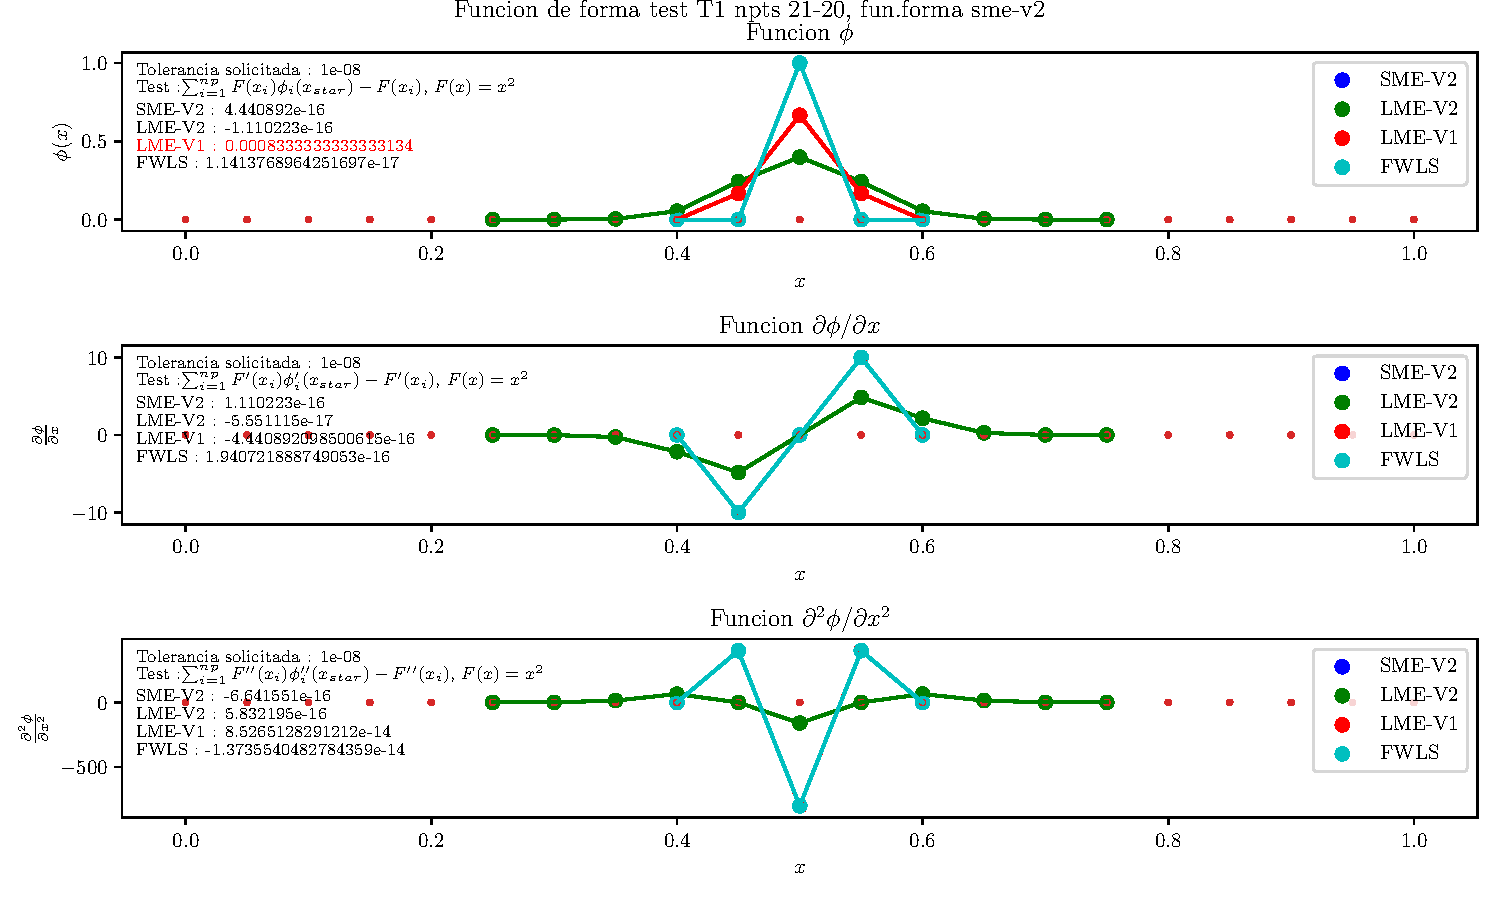
\includegraphics[width=1\textwidth]{./Imagenes/05/T1_21-20_regular_type-2_direct_10.pdf}
    \caption{Gráfica de las funciones de forma para una distribución regular} \label{fig:multiple_sf}
\end{figure}

\begin{figure}
    \centering
    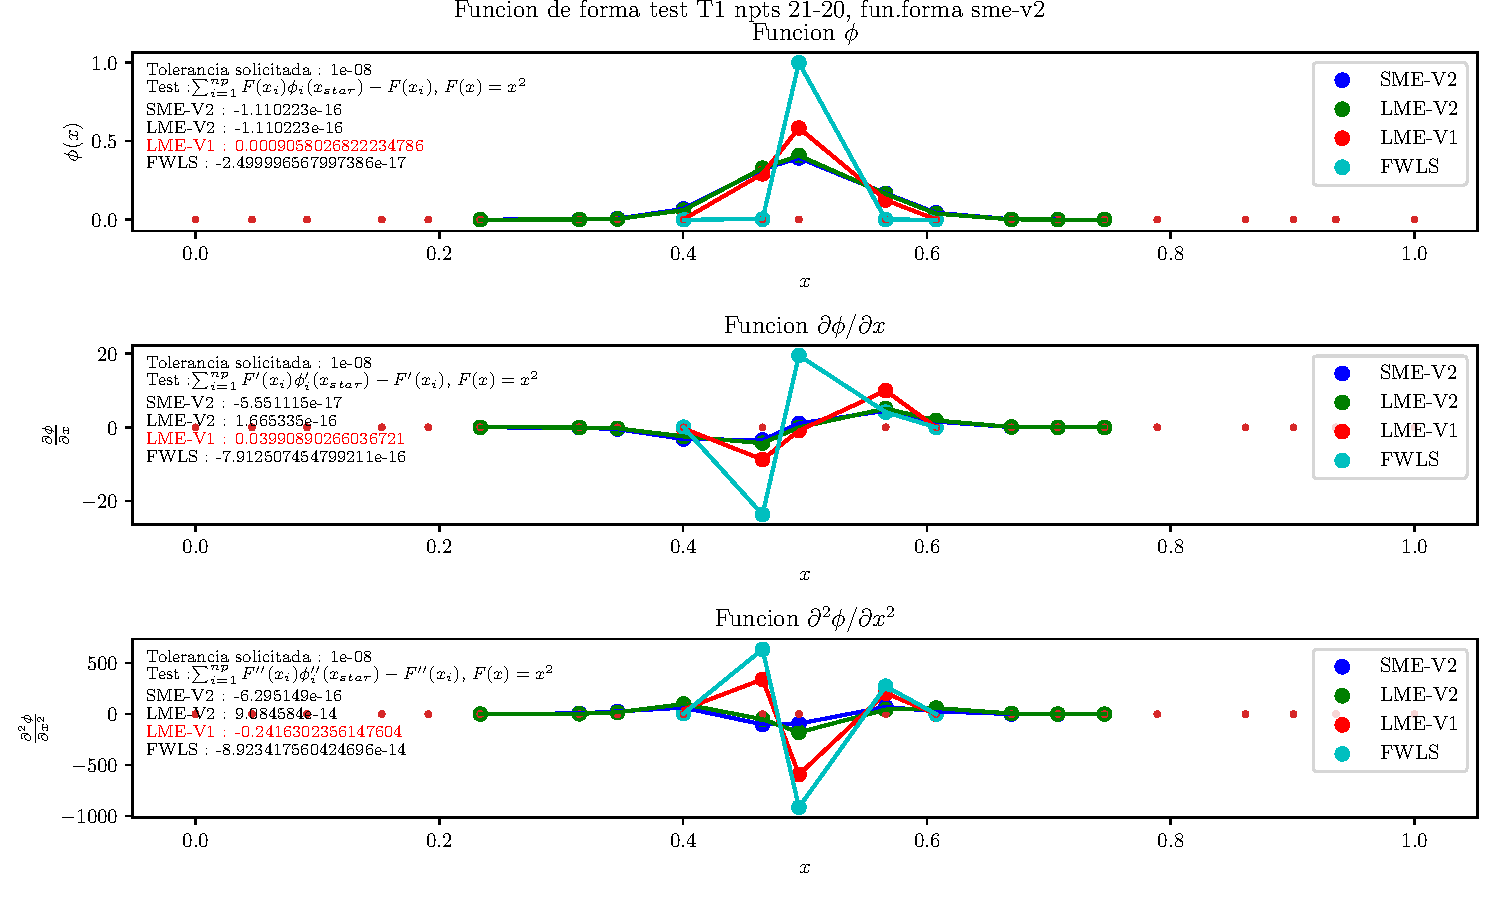
\includegraphics[width=1\textwidth]{./Imagenes/05/T1_21-20_irreg_type-2_direct_10.pdf}
    \caption{Gráfica de las funciones de forma para una distribución irregular} \label{fig:multiple_sf}
\end{figure}



%
\chapter{Resultados Obtenidos y Análisis}

( Hablar de los resultados )

%
\chapter{Conclusiones y Trabajo Futuro}

( Conclusiones, etc  )

%%
\appendix
%%%% Cap'itulos incluidos despues del comando \appendix aparecen como ap'endices
%%%% de la tesis.

\graphicspath{{./Imagenes/an1/}}
\chapter{Cálculo de Resultados para Bolund y Comparación Ciega}
\label{ch:apA}
%A modo de tener resultados comparables para el ejercicio de comparación ciega organizado por los desarrolladores del experimento de Bolund \citep{Bechmann2011}, se introducen ciertas métricas para la velocidad y para la energía cinética turbulenta.
%
%Para el caso de la velocidad, se adimensionaliza esta de la siguiente forma:
%\begin{equation}
%\Delta S_s = \frac{\overline{s} - \overline{s_0}}{\overline{s_0}},
%\end{equation}
%donde $\Delta S_s$ corresponde al \emph{Speedup} simulado, calculado en función de $\overline{s_0}$ que es un valor de referencia para la velocidad ubicado en un punto no perturbado por el terreno (en el experimento de Bolund se utiliza el valor en el mástil M0). Para los resultados presentados en esta tesis los valores de referencia se toman en las coordenadas (55.70313,12.0970) que caen dentro del dominio d08 de simulación.
%
%El valor de $\overline{s_0}$, operativamente, se toma como el promedio temporal entre las 12:00 y 15:00 horas y se calcula para cada nivel vertical del modelo.
%
%Con respecto a la energía cinética turbulenta, esta se adimensionaliza como:
%\begin{equation*}
%\Delta k_s = \frac{\overline{k}}{\overline{s_0^2}} - \frac{\overline{k_0}}{\overline{s_0^2}}.
%\end{equation*}
%Análogamente al caso anterior, $\overline{k_0}$ es un valor de referencia para la energía cinética turbulenta en el punto del dominio donde hay flujo no perturbado.
%
%De manera referencial, los desarrolladores presentan los siguientes resultados para su comparación ciega de modelos numéricos:
%\newpage
%
%\begin{figure}[H]
%	\centering
%	\includegraphics[width=0.85\linewidth,trim={2.7cm 14.3cm 2.0cm 2cm},clip]{bolund1.pdf}%
%	\caption{Perfil del viento no perturbado en el punto referencial M0 (ver Figura \ref{fig:05_terreno_bolund}). En línea negra está el perfil entregado por los desarrolladores (para utilizar como condición de borde) y el resto corresponde a distintos modelos. La línea sólida roja corresponde a simulaciones LES.}
%	\label{fig:an1_m0}
%\end{figure}
%
%\begin{figure}[H]
%	\centering
%	\includegraphics[width=0.9\linewidth,trim={1.7cm 12.3cm 0.9cm 2cm},clip]{bolund2.pdf}%
%	\caption{Speedup medido y simulado a través de la sección transversal a $240^\circ$. Arriba: valores para $z=5$ [m]. Abajo: valores para $z=2$ [m].}
%	\label{fig:an1_speedup}
%\end{figure}
%
%\newpage
%\vspace*{\fill}
%\begin{figure}[H]
%	\centering
%	\includegraphics[width=1.0\linewidth,trim={2.7cm 14.4cm 1.9cm 2cm},clip]{bolund3.pdf}%
%	
%	\includegraphics[width=1.0\linewidth,trim={2.7cm 6.0cm 1.9cm 10.3cm},clip]{bolund3.pdf}%
%	\caption{Perfil de speedup medido y simulado en los distintos mástiles M1-M4.}
%	\label{fig:an1_speed_masts}
%\end{figure}
%\vspace*{\fill}
%\newpage
%\vspace*{\fill}
%\begin{figure}[H]
%	\centering
%	\includegraphics[width=1\linewidth,trim={1.7cm 12.3cm 0.8cm 2cm},clip]{bolund4.pdf}%
%	
%	\caption{$\Delta k$ medido y simulado a través de la sección transversal a $240^\circ$. Arriba: valores para $z=5$ [m]. Abajo: valores para $z=2$ [m].}
%	\label{fig:an1_delta_tke}
%\end{figure}
%\vspace*{\fill}
%\newpage
%\vspace*{\fill}
%\begin{figure}[H]
%	\centering
%	\includegraphics[width=1\linewidth,trim={2.7cm 3.8cm 1.9cm 12.5cm},clip]{bolund4.pdf}%
%	
%	\includegraphics[width=1\linewidth,trim={2.7cm 14.3cm 1.9cm 2cm},clip]{bolund5.pdf}%
%	\caption{Perfil de $\Delta k$ medido y simulado en los distintos mástiles M1-M4.}
%	\label{fig:an1_delta_tke_mast}
%\end{figure}
%\vspace*{\fill}

\chapter{Incorporación de Bases de Datos de Alta Resolución}
%La utilización del modelo WRF con dominios anidados hasta resoluciones del orden de los metros, exige la implementación de bases de datos no nativas del software para la información estática (orografía y uso de suelo) en los dominios.
%
%En este anexo se presenta el mapeo de las bases de datos descritas en las Tablas \ref{tab:05_caract_hov} y \ref{tab:05_caract_bol}, y una breve explicación acerca de cómo se manejaron las bases de datos.
%
%Con respecto a la manipulación de los datos, esta se realizó a través un software GIS (\emph{Geographic Information System}) y la librería GDAL para la conversión de la extensión de los archivos. En particular, se utilizó el programa QGIS que es gratuito y de código libre. Los trabajos hechos incluyen:
%\begin{itemize*}
%	\item Conversión de los datos Corine (CLC12) al formato de clasificación USGS24 y su correspondiente transformación a formato binario.
%	\item Transformación del datúm de la base de datos orográfica entregada por la campaña de medición de Bolund a WGS84.
%	\item Creación de la base de datos para el uso de suelo en Bolund según lo declarado por la campaña \citep{3d4285ac04444eb3b9775baf9af052c6}.
%	\item Refinamiento de los datos CLC12 (hecho de manera manual) para ajustar al contorno de la colina de Bolund.
%	\item Ajuste de alturas de la base de datos orográfica de Bolund para su correcta implementación en WPS (fijar la altura de agua en $z=0$).
%	\item Transformación de todos los datos a formato binario para la lectura del WPS.
%\end{itemize*}
%
%A continuación se presentan algunos ejemplos de códigos simples desarrollados para las tareas descritas.
%
%Código en QGIS para la transformación de CLC12 a USGS24 según \cite{Pineda2004}:
%\lstset{style=consola}
%\begin{lstlisting}
%("test@1"<=11)*1+("test@1"=12)*2+("test@1"=13)*3+("test@1"=14)*3+
%("test@1"=15)*6+("test@1"=16)*6+("test@1"=17)*6+("test@1"=18)*2+
%("test@1"=19)*6+("test@1"=20)*6+("test@1"=21)*6+("test@1"=22)*6+
%("test@1"=23)*11+("test@1"=24)*14+("test@1"=25)*15+("test@1"=26)*7+
%("test@1"= 27)*9+("test@1"=28)*9+("test@1"=29)*9+("test@1"=30)*19+
%("test@1"=31)*19+("test@1"=32)*19+("test@1"=33)*19+("test@1"=34)*24+
%("test@1"=35)*17+("test@1"=36)*17+("test@1"=37)*17+("test@1"=38)*17+
%("test@1"=39)*17+("test@1"=40)*16+("test@1"=41)*16+("test@1"=42)*16+
%("test@1"=43)*16+("test@1">=44)*16
%\end{lstlisting}
%Código GDAL para la generación de uso de suelo en Bolund a partir de su orografía:
%\begin{lstlisting}
%gdal_calc.py -A bolund_rought_displaced_wgs84.tif --outfile=result.tif 
%--calc="16*(A<0.01)+2*(A>0.01)"
%\end{lstlisting}
%Código GDAL para la conversión del uso de suelo de Bolund de GeoTIFF a binario:
%\begin{lstlisting}
%gdal_translate -of ENVI -ot Int16 result.tif BOLUND_LANDUSE.bil
%\end{lstlisting}
%Código GDAL para correjir los valores indefinidos generados por la rotación del datum:
%\begin{lstlisting}
%gdal_calc.py -A BOLUND_LANDUSE.bil --outfile=BOLUND_LANDUSE2.bil 
%--calc="(A==32767)*16+(A<32767)*A"
%\end{lstlisting}
%
%Finalmente las bases de datos introducidas de orografía y uso de suelo se ven en el modelo como las Figuras \ref{fig:dominios_hov} y \ref{fig:dominios_bol}. Notar que el color amarillo para la categoría de uso de suelo significa la incorporación manual del $z_0$ según la información presente en las publicaciones correspondientes para cada dominio.
%\newpage
%\vspace*{\fill}
%\begin{figure}[H]
%	\centering
%	\includegraphics[width=0.25\linewidth,page=1,trim={2cm 6.5cm 1cm 3.5cm},clip]{Imagenes/05/hov_domain.pdf}%
%	\includegraphics[width=0.25\linewidth,page=2,trim={2cm 6.5cm 1cm 3.5cm},clip]{Imagenes/05/hov_domain.pdf}%
%	\includegraphics[width=0.25\linewidth,page=3,trim={2cm 6.5cm 1cm 3.5cm},clip]{Imagenes/05/hov_domain.pdf}%
%	\includegraphics[width=0.25\linewidth,page=4,trim={2cm 6.5cm 1cm 3.5cm},clip]{Imagenes/05/hov_domain.pdf}%
%	
%	\bigskip
%	\includegraphics[width=0.25\linewidth,page=5,trim={2cm 6.5cm 1cm 3.5cm},clip]{Imagenes/05/hov_domain.pdf}%
%	\includegraphics[width=0.25\linewidth,page=6,trim={2cm 6.5cm 1cm 3.5cm},clip]{Imagenes/05/hov_domain.pdf}%
%	\includegraphics[width=0.25\linewidth,page=7,trim={2cm 6.5cm 1cm 3.5cm},clip]{Imagenes/05/hov_domain.pdf}%
%	\includegraphics[width=0.25\linewidth,page=8,trim={2cm 6.5cm 1cm 3.5cm},clip]{Imagenes/05/hov_domain.pdf}%
%	
%	\bigskip
%	\includegraphics[width=0.25\linewidth,page=9,trim={2cm 6.5cm 1cm 3.5cm},clip]{Imagenes/05/hov_domain.pdf}%
%	\includegraphics[width=0.25\linewidth,page=10,trim={2cm 6.5cm 1cm 3.5cm},clip]{Imagenes/05/hov_domain.pdf}%
%	\includegraphics[width=0.25\linewidth,page=11,trim={2cm 6.5cm 1cm 3.5cm},clip]{Imagenes/05/hov_domain.pdf}%
%	\includegraphics[width=0.25\linewidth,page=12,trim={2cm 6.5cm 1cm 3.5cm},clip]{Imagenes/05/hov_domain.pdf}%
%	
%	\bigskip
%	\includegraphics[width=0.25\linewidth,page=13,trim={2cm 6.5cm 1cm 3.5cm},clip]{Imagenes/05/hov_domain.pdf}%
%	\includegraphics[width=0.25\linewidth,page=14,trim={2cm 6.5cm 1cm 3.5cm},clip]{Imagenes/05/hov_domain.pdf}%
%	
%	\caption{Orografía (MSNM) y uso de suelo (categoría USGS24) de alta resolución para cada uno de las mallas anidadas (d01-d07) en Høvsøre.}
%	\label{fig:dominios_hov}
%\end{figure}
%\vspace*{\fill}
%\newpage
%\vspace*{\fill}
%\begin{figure}[H]
%	\centering
%	\includegraphics[width=0.25\linewidth,page=1,trim={2cm 6.5cm 1cm 3.5cm},clip]{Imagenes/05/bol_domain.pdf}%
%	\includegraphics[width=0.25\linewidth,page=2,trim={2cm 6.5cm 1cm 3.5cm},clip]{Imagenes/05/bol_domain.pdf}%
%	\includegraphics[width=0.25\linewidth,page=3,trim={2cm 6.5cm 1cm 3.5cm},clip]{Imagenes/05/bol_domain.pdf}%
%	\includegraphics[width=0.25\linewidth,page=4,trim={2cm 6.5cm 1cm 3.5cm},clip]{Imagenes/05/bol_domain.pdf}%
%	
%	\bigskip
%	\includegraphics[width=0.25\linewidth,page=5,trim={2cm 6.5cm 1cm 3.5cm},clip]{Imagenes/05/bol_domain.pdf}%
%	\includegraphics[width=0.25\linewidth,page=6,trim={2cm 6.5cm 1cm 3.5cm},clip]{Imagenes/05/bol_domain.pdf}%
%	\includegraphics[width=0.25\linewidth,page=7,trim={2cm 6.5cm 1cm 3.5cm},clip]{Imagenes/05/bol_domain.pdf}%
%	\includegraphics[width=0.25\linewidth,page=8,trim={2cm 6.5cm 1cm 3.5cm},clip]{Imagenes/05/bol_domain.pdf}%
%	
%	\bigskip
%	\includegraphics[width=0.25\linewidth,page=9,trim={2cm 6.5cm 1cm 3.5cm},clip]{Imagenes/05/bol_domain.pdf}%
%	\includegraphics[width=0.25\linewidth,page=10,trim={2cm 6.5cm 1cm 3.5cm},clip]{Imagenes/05/bol_domain.pdf}%
%	\includegraphics[width=0.25\linewidth,page=11,trim={2cm 6.5cm 1cm 3.5cm},clip]{Imagenes/05/bol_domain.pdf}%
%	\includegraphics[width=0.25\linewidth,page=12,trim={2cm 6.5cm 1cm 3.5cm},clip]{Imagenes/05/bol_domain.pdf}%
%	
%	\bigskip
%	\includegraphics[width=0.25\linewidth,page=13,trim={2cm 6.5cm 1cm 3.5cm},clip]{Imagenes/05/bol_domain.pdf}%
%	\includegraphics[width=0.25\linewidth,page=14,trim={2cm 6.5cm 1cm 3.5cm},clip]{Imagenes/05/bol_domain.pdf}%
%	
%	\bigskip
%	\includegraphics[width=0.25\linewidth,page=15,trim={0cm 6.5cm 1cm 3.5cm},clip]{Imagenes/05/bol_domain.pdf}%
%	\includegraphics[width=0.25\linewidth,page=16,trim={0cm 6.5cm 1cm 3.5cm},clip]{Imagenes/05/bol_domain.pdf}%
%	
%	\caption{Orografía (MSNM) y uso de suelo (categoría USGS24) de alta resolución para cada uno de las mallas anidadas (d01-d08) en Bolund.}
%	\label{fig:dominios_bol}
%\end{figure}
%\vspace*{\fill}

\chapter{Eficiencia Computacional de las Simulaciones}
\label{apB}
%Las simulaciones se llevaron a cabo en servidores configurados especialmente para ejecutar el código WRF de manera paralela haciendo uso de todos los núcleos y recursos disponibles. En específico se utilizaron dos servidores distintos: S1 es el servidor utilizado para correr las simulaciones correspondientes al caso I de terreno plano en Høvsore y S2 es el servidor utilizado para correr el caso II de terreno complejo en Bolund. Otros recursos computacionales adicionales fueron utilizados también para llevar a cabo distintos análisis de sensibilidad para diversos parámetros y otras pruebas varias las cuales no se detallan en este documento. Las especificaciones técnicas de S1 y S2 se presentan en la Tabla \ref{tab:an3_s12}.
%
%\begin{table}[H]
%	\caption{Específicaciones técnicas de los recursos computacionales utilizados.}\label{tab:an3_s12}
%	\centering\resizebox{\textwidth}{!}{
%	\begin{tabular}{lcc}
%		\toprule
%		Servidor 				& S1	&	S2	\\
%		\midrule
%		CPU			 			& Intel Xeon CPU E5-2609 v2@2.50Ghz & Intel Xeon Silver 4110 CPU @ 2.10GHz  \\
%		\# Cores				& 8 & 32  \\
%		Arquitectura            & x86\_64  & x86\_64  \\
%	 	RAM			 			& 55Gb & 126Gb  \\
%		HDD			 			& 1Tb & 2Tb  \\
%		OS			 			& Scientific Linux 7.2 & Debian 9  \\
%		\bottomrule
%	\end{tabular}}
%\end{table}
%
%Para cada servidor se registraron los tiempos de pared a través de un bot de \emph{Telegram} el cual registraba de manera automática e inmediata la fecha y hora a la cual cada simulación comenzaba o terminaba. Los registros de estos tiempos se resumen en la Tabla \ref{tab:an3_tiempos}.
%\newpage
%\begin{table}[H]
%	\caption{Tiempos de cálculo para cada experimento.}\label{tab:an3_tiempos}
%	\centering\resizebox{\textwidth}{!}{
%	\begin{tabular}{lccccc}
%		\toprule
%		Caso 				& Fecha Inicio	&	Fecha Término & $T_w$ [h] &	$\Delta t$ [h] & Incremento	\\
%		\midrule
%		Høvsøre s/DA		& 25/02/2019 17:30 & 04/03/2019 01:28 & 151,97 & -- & --  \\
%		Høvsore c/ DA		& 13/03/2019 23:13 & 19/03/2019 00:49 & 121,60 & -30,37 & -19.98\% \\
%		Bolund s/DA			& 12/02/2019 22:22 & 20/03/2019 08:35 & 850,22 & -- & -- \\
%		Bolund c/ DA		& 25/04/2019 22:58 & 24/05/2019 09:44\footnotemark & 662,02 & -188,20 & -22,14\% \\
%		\bottomrule
%	\end{tabular}}
%\end{table}
%
%Acá $T_w$ es el tiempo de cálculo efectivo (tiempo de pared) y $\Delta t$ corresponde al aumento en este debido a la incorporación del proceso de asimilación de datos. El incremento se calcula como $\Delta t/T_{w0}$, donde el subíndice 0 índica la simulación sin asimilación de datos.
%
%Como se puede apreciar en la Tabla \ref{tab:an3_tiempos}, el proceso de asimilación de datos presenta mejoras significativas en términos del tiempo de cálculo, lo que es esperanzador para una implementación efectiva y efectiva de la solución propuesta. 
%
%\footnotetext{Por motivos externos la simulación estuvo detenida desde el 02/05/2019 14:43 hasta el 03/05/2019 12:28, por lo cual se considera esta detención en el cálculo.}

%

%%% Incluir la bibliograf'ia. Mirar el archivo "biblio.bib" para m'as detales
%%% y un ejemplo.
%

\nocite{*}     %incluir en la bibliografia articulos no citados
\bibliography{Bibliografia/biblio}
\end{document}
